\documentclass[11pt,journal,compsoc]{IEEEtran}

\usepackage{amsmath}

\usepackage{graphicx}

\usepackage{url}

\usepackage{hyperref}

\usepackage{enumitem}

\usepackage{amssymb}

\usepackage{indentfirst}

\setlength{\parindent}{0em}

\usepackage{float}

\usepackage{minted}

\usemintedstyle{colorful}

\setminted{
    frame=lines,
    breaklines,
    fontsize=\footnotesize
}

\begin{document}


\section{Processors \& Memories}


\subsection{Von Neumann Principle}

Programs and data are stored in a single, independent storage unit, memory, accessed via a common bus. They are physically identical, and the computer processes them according to instructions that can be easily reprogrammed.


\subsection{Von Neumann Loop}

\begin{enumerate}
    \item CPU Fetch instruction from memory Fetch
    \item Decode to determine operation Decode
    \item Execute Execute
    \item Fetch from memory
    \item Write back to memory
\end{enumerate}

The CPU alternates between fetching instructions and data, reducing speed.


\subsection{Von Neumann Architecture}

Memory, operators, controllers, input devices, and output devices comprise a computer's five parts. Operators and controllers are collectively known as the central processing unit.


\subsection{Harvard}

This architecture uses two different memories for instructions and data, accessed on different buses, which is faster and more costly.


\subsection{CISC}

Complex / Reduced Instruction Set Computer

Each instruction in a complex instruction set performs several low-end operations; the number of instructions is large and complex, and the cycle time is long, making it more suitable for complex operations, where simple operations may waste time.

Reason: registers are expensive, make a single instruction do as much work as possible


\subsection{RISC}

Thin instruction sets are optimized for pipelined processors, with fewer instructions, shorter cycles, better parallel execution, more efficient compilers, and cheaper and more energy efficient.

x86 has hardware acceleration for simple instructions.

ARM V7 and before do not have AES.


\subsection{Commands}

A set of binary codes instructs the processor to perform a specific operation, containing both OpCode and Operand. Assembly.


\subsection{Registers}

Memory is used inside the CPU to hold temporary data. very fast and small. x86-64 architecture has 16 general-purpose registers.

CPU $\leftrightarrow$ register $\leftrightarrow$ cache $\leftrightarrow$ memory


\subsection{Pipeline}

Instruction pipelining, where each instruction is broken down into multiple steps and different instructions can be executed in parallel at each stage, thus enabling several instructions to be processed in parallel. Instructions are still executed sequentially one by one, and a complete instruction can be executed in one clock cycle. While one instruction is Executing, another instruction can start executing Decode, and so on.


\subsection{Superscalar}

There are multiple pipelines in a single core, executing multiple instructions in a single clock cycle and pipelining multiple instructions in parallel.


\subsection{Memories}


\subsubsection{By physical structure}

\begin{description}
    \item[SRAM] Field-Effect Transistor, No Refresh, Very Fast, Expensive, CPU Cache

    \item[DRAM] Capacitance, Cycle Refresh, Memory

    \item[ROM] Read-Only

    \item[Programmable ROM] Fuse inside, and use electric current to blow it to write data. Once blown, cannot be recovered.

    \item[Erasable PROM] High voltage is used to write data and has a transparent window that erases data when exposed to ultraviolet light.

    \item[OneTime PROM] Same as EPROM but without the transparent window.

    \item[Electrically EPROM] Uses a high electric field to erase.

    \item[Flash] NAND ($! \&$ SSD) and NOR ($! \|$ BIOS) type, limited lifetime, slower
\end{description}


\subsubsection{By organization}

\begin{description}
    \item[Serial] e.g. Magnetic Tape, high density, slow, no random access.

    \item[Parallel] e.g. Disk, reads and writes multiple bits simultaneously.

    \item[Distributed] Information is stored in multiple independent and non-interfering devices, reliability, scalability

    \item[Hierarchical] high efficiency, e.g. Cache -> RAM -> ROM
\end{description}


\subsubsection{By type of visit}

\begin{description}
    \item[Direct Memory Access] DirectStorage without going through the CPU, e.g., graphics cards

    \item[Sequential Access Memory] Magnetic Tape

    \item[Random Access Memory] memory
\end{description}


\section{Peripherals \& Storage \& I/O}


\subsection{Storage}

\subsubsection{By Construction}

\begin{description}
    \item[Solid] SSD, Flash: quick

    \item[Optical] CD, use Laser

    \item[Magnetic] HDD, Tape, Floppy: large capacity
\end{description}

\subsubsection{By Operation Principle}

\begin{description}
    \item[RAM] Volatile
    \item[ROM] Non-Volatile
    \item[Sequential]
\end{description}


\subsection{Peripherals}

\subsubsection{By Functionality}

\begin{description}
    \item[Input] Keyboard, Mouse
    
    \item[Output] Monitor, Speaker

    \item[Storage] Flash Drive

    \item[Network] Router, Switch
\end{description}

\subsubsection{By Means}

\begin{description}
    \item[Wired]
    \item[Wireless]
\end{description}

There's also Bidirectional.


\subsection{Bus}

is physical pathways used by CPU and other devices to communicate.


\subsubsection{Data}

CPU \leftrightarrow RAM

CPU \leftrightarrow I/O Devices

Transmit data, width determines how many bits are transmitted at a time, 8 - 64 bits common


\subsubsection{Address}

Communicates physical address, width determines size of memory addressed


\subsubsection{Control}

Signals for controlling CPUs and devices: read/write, clock, interrupt, reset, etc.


\subsection{I/O}

handling is the process of managing the communication between CPU and devices.


\subsubsection{Programmed}

Simplest, basic, inefficient. CPU directly controls data transfers between I/O devices and memory, polling.


\subsubsection{IRQ}

Interrupt-Request. sends an interrupt request to the CPU when the I/O is ready and handles the request


\subsubsection{Direct Memory Access}


\subsection{Protocols}

Methods of transmitting data


\subsubsection{Parallel}

All signal lines transmit data at the same time, leading to signal interference (crosstalk). As the transmission rate increases, clock synchronization and timing control become more challenging.

\begin{description}
    \item[Centronics] Enhanced Parallel Port: Used for printer communication, featuring an 8-bit data bus and several control signals, with 25 pins.
    
    \item[Peripheral Component Interconnect] (PCI): Connects peripheral devices with a 32-bit bus and a speed of 133 MB/s.
\end{description}


\subsubsection{Serial}

Transmitting one bit at a time, data travels along a single channel, reducing interference and improving quality with differential signals. Increasing the number of lanes enhances the speed.

Differential signaling: Two lines, one positive and one negative, use voltage differences to obtain data.

\begin{description}
    \item[Recommended Standard 232] (RS-232): Uses one data line for both transmission and reception, with control lines for handshaking and flow control; commonly used in industrial applications.
    
    \item[High-Definition Multimedia Interface] (HDMI): Also known as DP (DisplayPort).
    
    \item[PCI Express]: Represented by x32 indicating the number of lanes, achieving 32 GT/s per lane.
\end{description}


\subsubsection{Universal Serial Bus}

Simultaneously provides power and communication, plug-and-play functionality, 40 Gbps speed, Thunderbolt compatible.

\begin{description}
    \item[Host Communication] Host manages and controls data transmission.
    
    \item[Hierarchical Structure] ~
    
        \begin{itemize}
            \item Physical: Interface shape, power, etc.
            \item Link: Establishes and maintains communication.
            \item Protocol: Format, etc.
            \item Transport: Packages data.
            \item Session: Management.
            \item Application: Handles driver requests.
        \end{itemize}
    
    \item[Data Packets] Basic units of transmission, including Token, Data, and Handshake.
    
    \item[Transfer Modes] ~
    
        \begin{itemize}
            \item Control: Device configuration, status queries, command execution.
            \item Bulk: Large data, high speed, high latency.
            \item Interrupt: Low latency, small data, real-time, slow (e.g., for mice).
            \item Isochronous: Audio and video, fixed rate and latency, may drop packets.
        \end{itemize}
    
    \item[Initialization] Identify devices, query information, allocate addresses, select configurations.
\end{description}


\section{Operating Systems}

Software that manages hardware, providing basic services for programs and acting as an intermediary between users and hardware.


\subsection{Classification}

\begin{description}
    \item[Batch] Automates the execution of a series of tasks (common in early large computers).
    
    \item[Time-Sharing] Allows multiple users to share resources, uses time-slicing to allocate time segments to each user for concurrent use.
    
    \item[Real-Time] Immediately responds to events; failures classified as Hard (missed deadlines) or Soft (tolerable).
    
    \item[Distributed] Utilizes a cluster of supercomputers for multiple tasks.
    
    \item[Embedded] Used in the Internet of Things (IoT).
\end{description}


\subsection{Functionality}

\begin{description}
    \item[Process Management] Allocates CPU time, manages priorities.
    
    \item[Memory Management] Utilizes virtual memory, allocates and bounds memory.
    
    \item[File System] Manages space allocation, controls access, maintains integrity.
    
    \item[Device Management] Provides standardized interfaces.
    
    \item[User Interface] Command Line Interface (CLI) / Graphical User Interface (GUI).
    
    \item[Security] Authentication / Authorization.
    
    \item[Networking] Inter-process and network communication.
    
    \item[Error Handling]
\end{description}


\subsection{Process \& Scheduling}

Ensures efficient resource utilization, providing a responsive and efficient environment for users.


\subsubsection{Process Management}

Creation, execution, termination.

\begin{description}
    \item[Process] An executing program, consisting of code, data, and a set of resources.
    
    \item[Control Block] Contains process information, such as ID, status, priority, memory usage, etc.
    
    \item[States] Examples include ready, running, waiting, terminated.
    
    \item[Scheduler] Determines which process from the ready queue should execute at a specified time, based on policies.
\end{description}


\subsubsection{Scheduling Methods}

\begin{description}
    \item[First-Come, First-Served] Assigns CPU time to the first process in the queue; not ideal for interactive use and may lead to long waits for some processes.
    
    \item[Shortest Job Next] Minimizes average waiting time but may lead to long waits for long processes.
    
    \item[Round Robin] Allocates a fixed time quantum to each process, balancing fairness and efficiency, suitable for interactive use.
    
    \item[Priority Scheduling] Executes higher-priority processes first to ensure responsiveness.
    
    \item[Multilevel Queue Scheduling] Uses separate queues for each priority level, often combined with other methods.
    
    \item[Multilevel Feedback Queue] Similar to the above, dynamically adjusts process priority based on behavior, improving efficiency and responsiveness (e.g., for I/O-bound processes).
\end{description}


\subsubsection{Scheduling in Interactive}

Prioritizes foreground tasks for responsiveness.

\begin{description}
    \item[Preemptive Scheduling] Allows interrupting running processes to allocate time to higher-priority tasks, ensuring timely response to inputs.
    
    \item[Dynamic Priority Adjustment] Adjusts priority based on behavior and resources, such as giving bursty CPU-bound tasks higher priority.
    
    \item[Load Balancing] Distributes processes among multiple CPU cores to prevent overload.
    
    \item[Resource Reservation] Allocates CPU time for critical processes.
    
    \item[Adaptive Scheduling] Dynamically adjusts scheduling strategies based on the system's evolving environment.
\end{description}


\subsubsection{Aim \& Requirements}

\begin{description}
    \item[Fairness] Maintains stability and equality, preventing monopolies.
    
    \item[Efficiency] Minimizes overhead, maximizes throughput, reduces context switches, and avoids CPU starvation.
    
    \item[Responsiveness] Swiftly responds to high-priority events.
    
    \item[Predictability] Ensures processes are executed within reasonable time frames based on priority and resource requirements, critical for real-time systems.
    
    \item[Adaptability] Adapts to changing system conditions, such as varying loads or the addition of new processes.
\end{description}


\subsection{Memory}


\subsubsection{Management}

Effectively allocate, track, and manage memory blocks to allow multiple processes to share memory and execute concurrently. Ensure each process has necessary runtime resources, prevent fragmentation, and maintain process isolation.

\begin{description}
    \item[De/Allocation] Allocate when needed, deallocate after use to prevent leaks.
    
    \item[Organization] Divide memory into sections for different types such as code, data, and stack for efficient management.
\end{description}


\subsubsection{Relocation}

Adjust the memory addresses of code and data, enabling execution at different locations and effective sharing of limited memory among multiple processes.

\begin{description}
    \item[Static] Adjust addresses during compilation or linking, resulting in a product with fixed addresses. Programs can only load at specific addresses, providing simplicity and speed but lacking flexibility as they cannot be moved once loaded.
    
    \item[Dynamic] Adjust addresses at runtime. Calculate the difference between the actual and reference positions during loading, known as Relocation Constant or Base Address, added to references in each memory. Allows multiple programs to share the same memory space without conflicts.
\end{description}


\subsubsection{Protection}

Prevent programs from illegitimately accessing another program's memory, ensuring stability, security, and integrity. Maintains process isolation, protects sensitive data, and prevents system crashes due to unauthorized operations.

\begin{description}
    \item[Memory Management Unit] Hardware that maps virtual addresses to physical addresses. Checks process access permissions for real-time memory protection. If unauthorized access occurs, an exception is thrown, prompting the operating system to take action, such as terminating the process.
    
    \item[Memory Protection Unit] Hardware, especially in systems without MMU or simple systems. Defines regions with specific memory access permissions and checks whether processes have the required permissions.
    
    \item[Virtual Memory] Each process has its private address space, separated from the physical layer, providing additional protection. The OS manages the mapping between virtual memory and physical addresses.
    
    \item[Access Control] OS implements various access control rules, such as permission groups, to restrict process access to areas.
    
    \item[Address Space Layout Randomization] Randomizes the location of code and data in memory, making it harder for attackers to predict layouts and execute attacks like Buffer Overflows.
\end{description}


\subsubsection{Swapping}

Swapping is the operation of using disk space to expand or free up RAM space, a crucial part of virtual memory management. When RAM is insufficient, the OS may swap out or page out some infrequently used data. When needed again, it is swapped in to RAM. However, this can slow down the system, so the OS uses complex algorithms based on frequency, memory usage, etc., to determine which parts can and when to swap.

\subsubsection{Paging}

Divide virtual memory into fixed-size blocks, pages, and physical memory into corresponding frames. They typically have the same size, often a power of 2. The OS maintains Page Tables that map pages to frames for MMU queries.

Advantages:

\begin{description}
    \item[Efficient Allocation] Avoid external fragmentation and simplify operations through block allocation.
    
    \item[Virtual Memory] The foundation of implementation.
    
    \item[Protection] Each process has its own Page Table, allowing the OS to set permissions for each page.
    
    \item[Demand Paging] Load pages only when they are actually used.
\end{description}

Disadvantages:

\begin{description}
    \item[Management] Page Tables require additional memory and processing.
    
    \item[Translation] Mapping overhead.
    
    \item[Page Faults] Occur when referencing a page not in physical memory, requiring the OS to load it from disk, which is relatively slow.
\end{description}


\section{Network Architectures}


\subsection{Layers}


\subsubsection{Open Systems Interconnection}

\begin{enumerate}
    \item Physical
    
    Electrical signals, voltage, medium specifications
    
    \item Data Link
    
    Error correction, flow control, includes LLC and MAC sub-layers
    
    \item Network
    
    Routing and forwarding between different networks, addressing, congestion control, packet sorting, IP operates at this layer
    
    \item Transport
    
    Reliable end-to-end transmission, error checking, flow control, data segmentation, TCP and UDP
    
    \item Session
    
    Managing connections between applications, handling interruption recovery
    
    \item Presentation
    
    Handling data encryption, compression, converting to a format understandable by applications
    
    \item Application
    
    Providing interfaces, high-level protocols such as HTTP
\end{enumerate}


\subsubsection{Logical Link Control}

Provides an interface between the Physical and MAC layers

\begin{description}
    \item[Multiplexing] Adding a protocol identifier to allow multiple upper-layer protocols to share the same MAC
    
    \item[Error Control] While MAC primarily handles errors, LLC can also retransmit
    
    \item[Flow Control] Regulating the rate to prevent buffer overflow
\end{description}


\subsubsection{Media Access Control}

Manages how data is transmitted over the medium

\begin{description}
    \item[Addressing] Allocates a unique hardware address (48 bits) to each interface in a device for identifying and directing data flow
    
    \item[Framing] Encapsulates content from upper layers, including header (control, MAC address), payload, and trailer (checksum)
    
    \item[Error Detection] Uses various algorithms to detect damaged frames, discarding and retransmitting
    
    \item[Access Control] Avoids conflicts, efficiently utilizes bandwidth
\end{description}


\subsubsection{TCP/IP}

TCP/IP is a protocol suite that includes various protocols: UDP, TCP, ICMP, IP...

\begin{enumerate}
    \item Link (1, 2)
    \item Internet (3)
    \item Transport (4)
    \item Application (5, 6, 7)
\end{enumerate}


\subsection{Hardware}

\begin{description}
    \item[Network Interfaces] 1, network card, transmits data over the network medium, assigns MAC addresses
    
    \item[Repeaters] 1, repeater, amplifies signals, extends coverage
    
    \item[Bridges] 2, bridge, connects two independent network segments. Uses a filtering table to forward data based on MAC addresses
    
    \item[Hubs] 1, hub, connects multiple devices in a network, forwards data to all connected devices without filtering
    
    \item[Switches] 2, switch, connects multiple devices in a network, forwards and filters based on MAC addresses, more efficient than hubs
    
    \item[Routers] 3, router, connects multiple networks and forwards based on IP, uses routing algorithms to determine the best path, provides NAT, firewall, QoS, etc.
\end{description}


\subsection{Ethernet}

It is a wired Local Area Network (LAN) technology, a LAN communication standard, operating at the 1/2 layer.

\begin{description}
    \item[Topology] Star structure, devices connected to a central device, such as a switch.
    
    \item[Media] Supports various media, including Coaxial, Twisted-pair, Fiber-Optic, RJ-45 interface.
    
    \item[Speed] 100 M/1 G/10 G, etc.
    
    \item[Frame] Preamble, Destination/Source MAC address, EtherType (payload's protocol), Payload (data), Frame Check Sequence.
    
    \item[MAC] Before transmission, it listens to the idle channel; if multiple devices attempt transmission simultaneously, it waits for a random time before retrying.
\end{description}

\subsection{802.11 / WiFi}

\begin{description}
    \item[a] 5 GHz, 54 Mbps, less susceptible to interference, limited range.
    
    \item[b] 2.4 GHz, 11 Mbps, susceptible to interference, broad range.
    
    \item[g] 2.4 GHz, 54 Mbps.
    
    \item[n] 2.4 and 5 GHz, 600 Mbps, four Spatial streams, MIMO.
    
    \item[ac] 5 GHz, 6.93 Gbps, eight streams, Multi-User MIMO, simultaneous transmission to multiple devices, 160 MHz channel, 256-QAM.
    
    \item[ax] 2.4 and 5 GHz, 9.6 Gbps, OFDMA, BSS Color.
\end{description}

\subsubsection{Multiple Input Multiple Output}

Multiple antennas at the transmitter independently send signals, while at the receiver, multiple antennas receive and recover the original information, increasing throughput and range.

\subsubsection{Quadrature Amplitude Modulation}

Modulation method that modulates amplitude on two orthogonal carriers, typically sine waves with a phase difference of 90 degrees. Each constellation point on the constellation diagram corresponds to a signal in the transmitted signal set. The more constellation points, the greater the amount of information that can be transmitted.

\subsubsection{Orthogonal Frequency Division Multiple Access}

Divides a high-speed data stream into multiple low-speed data streams, transmitting in parallel on multiple orthogonal subcarriers.

\subsubsection{Basic Service Set Coloring}

Tagging used to differentiate signals from different networks. In high-density environments, signals from different APs can interfere with each other, reducing performance. By assigning a color identifier to each BSS, interference between adjacent wireless networks is reduced.

\subsection{Internet Protocol}

An unreliable, connectionless network protocol that does not guarantee delivery and does not establish a connection before sending data. Operates at the third layer, addressing, routing, packaging.

\subsubsection{IPv4}

Header minimum 20 bytes:

\begin{description}
    \item[Version] 4 bits.
    
    \item[Internet Header Length] 4.
    
    \item[Type of Service] 8.
    
    \item[Total Length] 16.
    
    \item[Identification] 16, important for fragmentation and reassembly.
    
    \item[Flags] 3, —, [1] reserved, [2] do not fragment, [3] more fragments.
    
    \item[Fragment Offset] 13, —, index of the fragment.
    
    \item[Time to Live] 8, maximum hops before discarding.
    
    \item[Protocol] 8, TCP 6, UDP 17.
    
    \item[Header Checksum] 16, recalculated and checked at each hop.
    
    \item[Source IP] 32.
    
    \item[Destination IP] 32.
    
    \item[Options / Padding] var.
\end{description}


\subsubsection{IPv6}

IPsec, Improved QoS, Stateless IP Configuration, Multicast, and Anycast

Fixed-length Header of 40 bytes:

\begin{description}
    \item[Version] 4, 6

    \item[Traffic Class] 8, QoS

    \item[Flow Label] 20, Marks sequences with the same QoS

    \item[Payload Length] 16

    \item[Next Header] 8, e.g., TCP header

    \item[Hop Limit] 8, TTL

    \item[Source IP] 128

    \item[Destination IP] 128
\end{description}


\subsection{Network Address Translation}

Types of NAT:

\begin{description}
    \item[Static] One-to-one fixed public network

    \item[Dynamic] One-to-one dynamic public network

    \item[Port Address Translation] Common, shared public network
\end{description}

NAT Behavior:

\begin{description}
    \item[Full Cone] Any external can communicate with the internal mapped port

    \item[Restricted Cone] Internal can communicate externally first

    \item[Port Restricted Cone] Same port number

    \item[Symmetric] Each connection is assigned a different IP and port
\end{description}


\subsection{Classless Inter-Domain Routing}

Classless Inter-Domain Routing, Classful: A (x.0.0.1), B (x.x.0.1), C (x.x.x.1)

Subnet mask distinguishes network and host parts. Binary representation of 255.255.255.0 is 11111111.11111111.11111111.00000000; 24 ones denote the network, 8 zeros denote the host. So, CIDR for 192.168.1.1 and 255.255.255.0 is 192.168.1.1/24.

127.0.0.0/8 is a network range with subnet mask 255.0.0.0, encompassing all IP addresses from 127.0.0.0 to 127.255.255.255.

127.0.0.1/32 is a single IP address with subnet mask 255.255.255.255, representing only one IP address, 127.0.0.1. Also known as the loopback address.


\subsection{Routing}

Routing is the process of selecting paths to send network traffic in a way that ensures packets reach their destination effectively and accurately.

Routing table is a data structure storing information about paths to different network destinations. When a router receives a packet, it looks up the destination IP address in its routing table to determine the next hop for forwarding the packet. It includes:

\begin{description}
    \item[Destination / Mask] Destination network, can be an address or a subnet

    \item[Protocol] Method of obtaining this routing information, e.g., Direct (0), Static (60), OSPF (10), etc.

    \item[Preference] Differentiates between routing protocols, lower values indicate higher reliability

    \item[Cost] If routes are received from the same protocol, compare costs; different protocols are not comparable, smaller values are preferable

    \item[Next Hop] Next node

    \item[Interface] Exit device
\end{description}


\subsubsection{Border Gateway Protocol}

A protocol for exchanging Network Layer Reachability Information between Autonomous Systems. When running within the same Autonomous System, it is referred to as Internal BGP; when operating between different Autonomous Systems, it is known as External BGP.

The routing device that sends BGP messages is called a Speaker. It receives or generates new routes and advertises them to other neighbors. BGP operates over TCP and has five message types: Open, Update, Notification (Stop), Keepalive, and Route-refresh.

\subsection{Transmission Control Protocol}

Header 20 bytes:

\begin{description}
    \item[Source / Dest Port] TCP does not record IP.
    \item[Sequence Number] Resolves reordering; the transmitted byte count increases.
    \item[Acknowledgement Number] Confirms receipt.
    \item[Flags] Packet type, manipulates the state machine.
    \item[Window] Sliding window, flow control.
\end{description}

\subsubsection{Handshake}

Transmission on the network is connectionless, only the connection state exists.

\begin{description}
    \item[Three-Way Handshake] SYN - SYN - ACK, synchronizes Initial Sequence Number, used to concatenate data. When the server is in the SYN-RCVD state but hasn't received the final ACK, it retries with exponentially increasing time intervals. A flood attack creates numerous SYN connections and brings down the SYN queue. This can be temporarily mitigated using tcp-syncookies: a special Seq Num is sent back based on Src Des and timestamp, normal connections return the SYN Cookie and establish the connection directly.
    \item[Four-Way Handshake] Essentially two FIN - ACK, with one side being passive. If both parties FIN simultaneously, enter the Closing state, waiting for Maximum Segment Lifetime (30s) * 2 to ensure the other party receives the ACK. This provides enough time to prevent confusion with subsequent new connections (some routers may cache IP packets, and if the connection is reused, delayed packets may be confused with new connections).
\end{description}

\subsubsection{Retransmission}

The ACK sent by the Receiver to the Sender can only confirm the largest continuously received packet. For example, sending 1 2 3 4 5 and receiving 1 2, then replying with ACK 3 (the expected next data). Subsequently, receiving 4 without 3:

\paragraph{Timeout} ~

When the Sender times out without receiving ACK 3, it either retransmits 3 or retransmits 3 4 5. Both solutions require waiting for the timeout, which could take a long time.

\paragraph{Fast Retransmit} ~

Instead of time-driven, if the sender consecutively receives the same ACK three times, it retransmits. For example, receiving 1, replying with ACK 2; receiving 3, replying with ACK 2; receiving 4 5, replying with ACK 2. Then retransmit 2 and reply with ACK 6. This solves the timing problem but does not indicate whether to retransmit just one or all remaining packets.

\paragraph{Selective ACK} ~

To address this, a SACK is added to the TCP header, reporting received data as a range. However, the Receiver has the right to renege data, so the Sender cannot rely entirely on SACK, and SACK consumes Sender resources.

\paragraph{Duplicate SACK} ~

Using SACK informs the Sender of which data has been received repeatedly, providing information about:

\begin{enumerate}
    \item Whether the sent packet is lost or the ACK packet is lost.
    \item Whether the Timeout is too short.
    \item If reordering occurs on the network, where sent packets arrive later.
    \item Whether the network is duplicating data packets.
\end{enumerate}

\subsubsection{Advertised-Window}

This field informs the Sender of the remaining buffer size available for receiving data. The Sender can adjust data transmission based on the Receiver's processing capacity, avoiding overwhelming the Receiver.

If the window becomes 0, the Sender periodically sends Zero Window Probes to the Receiver to detect the latest Window size. After a certain number of attempts, the connection is terminated.

Silly Window Syndrome occurs if the received window is too small; it is treated as zero until the Window Size >= MSS. If network packets can fill the Maximum Transmission Unit, the full bandwidth can be utilized, resulting in the Max Segment Size. For programs that require small packets, such as SSH, Nagle is disabled.


\subsubsection{Congestion Handling}

TCP is not a selfish protocol; when congestion occurs, it sacrifices itself.

\paragraph{Slow Start} ~

For newly joined connections, it gradually increases speed.

\begin{enumerate}
    \item Congestion Window = 1, indicating the ability to transmit data of one MSS size.
    
    \item Increase Congestion Window (cwnd) for every received ACK.
    
    \item Double cwnd after each Round Trip Time.
    
    \item Slow Start Threshold acts as an upper limit. When cwnd >= ssthresh, it enters the congestion avoidance algorithm.
\end{enumerate}

\paragraph{Congestion Avoidance} ~

Typically, ssthresh is set to 65535 kb. When cwnd reaches this value:

\begin{enumerate}
    \item Increase cwnd by 1/cwnd upon receiving an ACK.
    
    \item Increase cwnd by 1 for every Round Trip Time.
\end{enumerate}

\paragraph{During Congestion} ~

If Retransmission Timeout is exceeded:

\begin{itemize}
    \item Set ssthresh = cwnd / 2.
    \item Set cwnd = 1.
    \item Enter slow start.
\end{itemize}

\subsection{User Datagram Protocol}

Header 8 bytes:

\begin{description}
    \item[Src Port] Used when a reply is needed.
    
    \item[Des Port] 
    
    \item[Length] 
    
    \item[Check Sum] 
\end{description}

Characteristics:

\begin{description}
    \item[Connectionless] Does not maintain connection state.
    
    \item[No Congestion Control] Tolerates data loss but not suitable for real-time applications with significant delay.
    
    \item[Unreliable] Lacks acknowledgment/retransmission mechanisms.
    
    \item[Datagram-oriented] Application-layer messages are sent directly to the IP layer with added headers, and vice versa, without merging or splitting.
\end{description}

Checksum:

UDP checksum is calculated using binary ones' complement arithmetic, similar to IP. However, UDP's checksum includes both a pseudo-header and data.

The pseudo-header includes:

\begin{description}
    \item[Src IP] 
    
    \item[Des IP] 
    
    \item[0] 
    
    \item[Protocol Number] 17
    
    \item[Datagram Length] 
\end{description}

\subsection{Quality of Service}

In limited bandwidth scenarios, QoS ensures the prioritization of important services during burst traffic.

Services can be categorized as:

\begin{description}
    \item[Real-time] Typically occupies fixed bandwidth with high stability requirements.
    
    \item[Non-real-time] Behavior is unpredictable, often causing burst traffic, leading to network quality degradation, congestion, increased latency, and packet loss.
\end{description}

Metrics: Bandwidth, Latency, Jitter, Packet Loss

\subsubsection{Service Models}

QoS models are not specific functionalities but rather schemes for end-to-end QoS design. End-to-end quality assurance is only possible when all network devices adhere to a unified QoS service model.

\begin{description}
    \item[Best-Effort] Simplest model where users can send any number of packets at any time. The network does its best to deliver without guarantees, suitable for low-demand services (default).
    
    \item[IntServ] Before sending packets, users must request specific QoS services from the network through signaling. The network reserves resources based on the request. Packet transmission begins after receiving confirmation.
    
    It uses the Resource Reservation Protocol to reserve resources along the entire path. The path can only be established if all network elements confirm.
    
    \item[DiffServ] Classifies traffic, providing different treatments. Similar types of services are aggregated and sent together, commonly used.
    
    Classification and aggregation occur at the network edge nodes. It uses various criteria such as source/destination addresses, protocol types, etc., to flexibly label packets. Other nodes only need to identify these labels for resource allocation and traffic control.
\end{description}


\subsection{Domain Name System}


\subsubsection{Hierarchy Structure}

Anonymous Root -> Top-level Domain (Generic / Country) -> Subdomains

The initial domain names always end with a dot, for example, www.kernel.org., indicating the root domain server.

\subsubsection{Domain Servers}

\begin{description}
    \item[Root] There are globally 13 different IP addresses for the highest-level domain servers, labeled from a to m. Managed by ICANN, utilizing Anycast.

    The Root NS knows the addresses of all top-level NS. When resolving aloen.to, it returns the Top NS for .to, then queries it for the DNS records of aloen.

    \item[Top-level] Responsible for resolving subdomains registered under that top-level domain.

    \item[Authoritative] Resolves subdomain queries.

    \item[Local] When a host issues a DNS query, it is first sent to the local NS.
\end{description}

DNS query with no result:

\begin{description}
    \item[Iterative] DNS server queries other servers.
    \item[Recursive] Returns another DNS server address.
\end{description}

\subsubsection{Common Record Types}

\begin{description}
    \item[Address] Maps to IPv4.

    \item[AAAA] IPv6.

    \item[Canonical NAME] Maps to another domain name, alias.

    \item[Mail Exchange] Points to mail servers.

    \item[NS] Specifies the authoritative domain name servers for the domain.

    \item[TXT] Stores arbitrary text information about the domain.

    \item[Pointer] IP reverse lookup.
\end{description}

\section{Network \& Security}

\subsection{Data Security}

Data Integrity, Confidentiality, and Availability.

\begin{description}
    \item[Encryption]
    \item[Access Control]
    \item[Backup]
    \item[Data Loss Prevention Tool] Detects and prevents illegal transfer and leakage of sensitive data.
    \item[Data Masking] Uses fictitious data to replace sensitive information.
\end{description}

\subsection{Service Security}

Protection against unauthorized access, damage, and vulnerabilities in applications and APIs.

\begin{enumerate}
    \item Regular vulnerability scanning and patching.
    \item Security testing during software development.
    \item Deployment of firewalls, IDS, IPS.
    \item Network segmentation.
    \item Secure configuration of devices and programs.
\end{enumerate}

\subsection{Physical Security}

Prevention of theft, damage, and unauthorized access.

\begin{description}
    \item[Security Facilities] Access control, surveillance cameras, alarms.
    \item[Access Control Systems] Card readers, biometrics, etc.
    \item[Security Personnel] Monitoring and patrol.
    \item[Environmental Control] Fire suppression systems, uninterruptible power supplies, air conditioning.
    \item[Asset Management \& Tracking]
\end{description}

\subsection{Security Risks of the Internet}

\begin{description}
    \item[Data Breaches] Unauthorized access leading to stolen identity information, financial losses, etc.
    \item[Malware] Viruses, worms, trojans, ransomware, spyware.
    \item[Social Engineering]
    \item[Distributed Denial of Service] Traffic attacks.
    \item[Insider Threats] Employee misuse of permissions.
\end{description}

\subsection{Classic Encryptions}

\begin{description}
    \item[Caesar Cipher] Offset substitution, each letter has a fixed replacement.
    \item[Vigenère] Consists of several Caesar ciphers with different offsets.
\end{description}


\subsection{Symmetric Cryptography}


\subsubsection{Advanced Encryption Standard}

The key length can be 128, 192, or 256 bits. The encryption process is briefly described as follows:

\begin{description}
    \item[SubBytes] Replace each byte of the plaintext with a fixed value found in the S-box.
    
    \item[ShiftRows] Circularly shift the bytes in each row to different columns.
    
    \item[MixColumns] Linearly transform the bytes in each column for confusion.
    
    \item[AddRoundKey] XOR each byte with the key for increased strength in each round.
\end{description}

128-bit key undergoes 10 rounds of encryption, 192-bit key undergoes 12 rounds, and 256-bit key undergoes 14 rounds.

In the inverse transformation, only AddRoundKey is the same as the encryption process.

\subsubsection{Substitution Box}

A substitution box, constructed from a fixed table, is used to map input bit sequences to output bit sequences. In AES, the S-box is meticulously crafted using various cryptographic principles and techniques to ensure good encryption and statistical properties. It contains 256 elements, each being an 8-bit binary number.

\subsection{RSA}

Three entities:

\begin{description}
    \item[Message] $M$
    
    \item[Ciphertext] Ciphertext $C$
    
    \item[Public / Private] Key
    
    \item[Encryption / Decryption] Algorithm
\end{description}

Key generation:

\begin{enumerate}
    \item Randomly choose two distinct prime numbers, $p = 103$, $q = 97$.
    
    \item $n = p * q = 9991$.
    
    \item Calculate Euler's totient function $\varphi(n) = (p - 1)(q - 1) = 9792$.
    
    \item Randomly choose $e = 1213$, where $e$ and $\varphi(n)$ are coprime ($\text{gcd}(a, b) = 1$) and $1 < e < \varphi(n)$.
    
    \item Find integer solutions to $ed - k\varphi(n) = 1$: $k = 510$, $d = 4117$.
    
    \item Public key: (e, n) = (1213, 9991).
    
    \item Private key: (d, n) = (4117, 9991).
\end{enumerate}

Encryption:

Let $M = 6$, resulting in $C = M^e \pmod{n}$.

$= 6^{1213} \pmod{9991} = 7863$.

Decryption:

$M = C^d \pmod{n} = 7683^{4117} \pmod{9991} = 6$.

\subsection{Diffie-Hellman}

Based on the difficulty of the Discrete Logarithm Problem.

\begin{enumerate}
    \item Both parties agree on large prime $G$ and primitive root $N$.
    
    $G = 13$, $N = 7$.
    
    \item Alice chooses a private integer $a = 2$.
    
    $A = G^a \pmod{N} = 13^2 \pmod{7} = 1$.
    
    \item Bob chooses a private integer $b = 3$.
    
    $B = 13^3 \pmod{7} = 6$.
    
    \item Both parties exchange $A$ and $B$.
    
    \item Alice computes the key using $B$.
    
    $K = B^a \pmod{N} = 6^2 \pmod{7} = 1$.
    
    \item Bob computes the key using $A$.
    
    $K = A^b \pmod{N} = 1^3 \pmod{7} = 1$.
\end{enumerate}

\subsection{Social Engineering}


\begin{description}
    \item[Phishing] Fraudulent Emails or Messages

    \item[Baiting] Fraudulent Winning Message

    \item[Tailgating] Tailgating the door

    \item[Impersonation] Impersonation

    \item[Dumpster Diving] Rummaging through a target's trash for information.

    \item[Shoulder Surfing] Observe from the side while the target enters sensitive information.

    \item[Reverse] Convince the target that they need help
\end{description}


\subsection{Brute-Force Attack}

\begin{description}
    \item[Dictionary] Common combinations

    \item[Hash Collision] Generating data with the same hash value as the original content, with added salt

    \item[Rainbow Table] Precomputed hash tables for looking up plaintext passwords
\end{description}


\subsection{Analytical Attack}

\begin{description}
    \item[Differential Cryptanalysis] Analyzing differences in multiple values to find algorithm patterns

    \item[Implementation] Finding software or hardware vulnerabilities, such as Buffer Overflow

    \item[Side-Channel]
\end{description}


\subsection{Firewall}

Monitors and controls network traffic based on a set of security rules; FW decides whether to allow traffic through. It can be embedded in hardware, software, or a combination to protect security. The untrusted network is typically the Internet. FW can also be used for content filtering; for example, schools can configure firewalls to prevent harmful content.

\begin{description}
    \item[Packet-filtering] Network layer, filters packets based on rules in the header, fast but lacks complex attack protection

    \item[Stateful] Network layer, tracks active connection states, provides finer control through context than packet filtering

    \item[Proxy-based] Application layer, acts as a proxy, performance may degrade when many people access simultaneously, causing latency

    \item[Next] In addition to the above functions, uses DPI to detect threats at a deeper level, identifying and blocking threats hidden in seemingly normal traffic
\end{description}


\subsubsection{Intrusion Detection Systems}

Monitors the operation status of networks and systems according to a set security policy, aiming to detect various attempted attacks, attack behaviors, or attack outcomes. It is a passive monitoring device. IDS should be connected to all links that all monitored traffic must pass through, as close to the attack source and as close to the protected resources as possible.

These positions are typically:

\begin{enumerate}
    \item On switches in the server area
    \item On the first switch after the Internet access router
    \item On LAN switches in the area of crucial protection
\end{enumerate}


\subsubsection{Intrusion Prevention Systems}

Complements antivirus software and firewalls, monitors network transmissions in serial deployment, and can instantly interrupt, adjust, or isolate some illegal transmission behaviors.

It can perform in-depth detection on each packet passing through, according to predefined security policies (protocol analysis tracking, feature matching, traffic statistical analysis, event correlation analysis, etc.). If a network attack hidden in the traffic is detected, defensive measures can be taken immediately based on the threat level.

These measures include:

\begin{enumerate}
    \item Alerting the management center
    \item Discarding the packet
    \item Terminating the application session
    \item Terminating the TCP connection
\end{enumerate}


\subsection{Demilitarized Zone}

A buffer zone located between the internal network and the external network, where some public resources, such as web servers, are placed.


\subsection{Wi-Fi Protected Access}

A replacement for Wired Equivalent Privacy (WEP).

\begin{description}
    \item[WPA-Personal] Uses a Pre-Shared Key; all devices use the same password for authentication

    \item[WPA-Enterprise] Uses the 802.1X authentication protocol; each user has their own username and password
\end{description}

\begin{description}
    \item[WPA1] Uses Temporal Key Integrity Protocol

    \item[WPA2] Uses stronger encryption algorithms (e.g., AES) and longer key lengths

    \item[WPA3] Introduces Simultaneous Authentication of Equals (SAE) and Dragonfly Key Exchange
\end{description}


\subsection{Fake Access Point}

By creating a fake Wi-Fi access point with the same or similar name, users are deceived into connecting, allowing for the theft of sensitive information.

The term "Wi-Fi" is meaningless and has no full form.

\section{Databases}

\url{https://Aloen.to/Database/MSSQL/MSSQL-Practice-Questions/}

\subsection{Data Independence}

Physical:

\begin{itemize}
    \item Programs are independent of data.
    \item Programs do not know how data is stored.
    \item Data is managed and stored by the DBMS.
    \item Physical storage changes do not require program changes.
\end{itemize}

Logical:

\begin{itemize}
    \item Programs are independent of the logical structure of the database.
    \item Changes in the logical structure of data do not require program changes.
\end{itemize}

Significance:

\begin{itemize}
    \item Low maintenance cost.
    \item Secure and stable.
    \item Structured.
    \item Hierarchical.
    \item Reduces redundancy.
    \item Easily scalable.
\end{itemize}

\subsection{Three-Level Schema}

\begin{description}
    \item[Physical]
    Internal schema (storage schema), physical (internal) level.
    
    Describes the storage format and physical structure of data on disk.

    \item[Conceptual]
    Conceptual schema (logical schema), conceptual (logical) level.
    
    Global view, describes the logical structure and characteristics, DDL.

    \item[External]
    External schema (user schema), user (view) level.
    
    User's view of data, a subset of the conceptual schema, includes the specific data that a particular user uses, DML.
\end{description}

\subsection{Relational Model}

\begin{figure}[H]
    \centering
    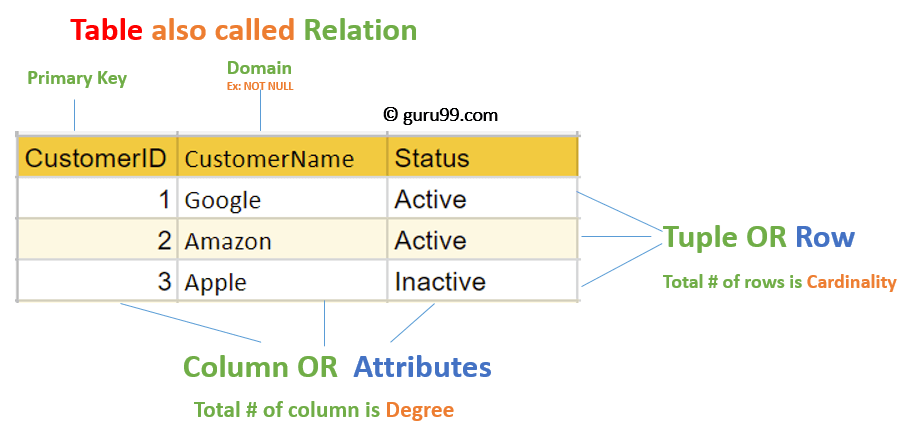
\includegraphics[width=\linewidth]{RelationalModel.jpg}
    \caption{Relational Model}
\end{figure}

\begin{description}
    \item[Attribute] Column
    \item[Relation] Table
    \item[Tuple] Row
    \item[Degree] Count(Column)
    \item[Cardinality] Count(Row)
    \item[Domain] Data types, constraints, etc.
    \item[Relation Key] Primary key, foreign key
    \item[Relation Schema] Table name and its columns
    \item[Relation Instance] Data in the table
\end{description}


\subsection{SQL}

Data Definition Language (DDL) Definition

\begin{itemize}
    \item CREATE
    \item ALTER
    \item DROP
    \item TRUNCATE
\end{itemize}

Data Manipulation Language (DML) Operations

\begin{itemize}
    \item INSERT
    \item UPDATE
    \item DELETE
\end{itemize}

Data Control Language (DCL) Permissions

\begin{itemize}
    \item GRANT
    \item REVOKE
\end{itemize}

Transaction Control Language (TCL) Transactions

\begin{itemize}
    \item COMMIT
    \item ROLLBACK
    \item SAVEPOINT
\end{itemize}

Data Query Language (DQL) Query

\begin{itemize}
    \item SELECT
\end{itemize}


\subsection{Indexes}

Clustered Index

\begin{itemize}
    \item Physical and logical order of rows are the same
    \item Only one per table
    \item Default for Primary Key
\end{itemize}

Non-clustered Index

\begin{itemize}
    \item Stores pointers to rows
    \item Default for UNIQUE
\end{itemize}

Covering Indexes

\begin{itemize}
    \item Index includes all the fields needed for a query
\end{itemize}


\subsection{Normalization}

Eliminating redundancy and inconsistent dependencies


\subsubsection{Inconsistency}

It is reasonable for a user to find the Address in the Customer table,
but it is not reasonable to find the Salary of the employee responsible for this customer here.
This should be looked up in the Employee table.

Inconsistent dependencies make data difficult to access

\begin{table}[H]
    \centering
    \begin{tabular}{|c|c|c|c|c|c|}
        \hline
        Student ID & Teacher & Consultation Room & Course 1 & Course 2 & Course 3 \\
        \hline
        S1 & T1 & R1 & C1 & C2 & C3 \\
        \hline
        S2 & T2 & R2 & C1 & C2 & C4 \\
        \hline
    \end{tabular}
\end{table}


\subsubsection{1NF}

Each field is atomic, does not contain other fields, and is not duplicated

\begin{itemize}
    \item Eliminate duplicate columns
    \item Create separate tables for related data
    \item Use a primary key to identify each group of related data
\end{itemize}

\begin{table}[H]
    \centering
    \begin{tabular}{|c|c|c|c|}
        \hline
        Student ID & Teacher & Consultation Room & Course \\
        \hline
        S1 & T1 & R1 & C1 \\
        \hline
        S1 & T1 & R1 & C2 \\
        \hline
        S1 & T1 & R1 & C3 \\
        \hline
        S2 & T2 & R2 & C1 \\
        \hline
        S2 & T2 & R2 & C2 \\
        \hline
        S2 & T2 & R2 & C4 \\
        \hline
    \end{tabular}
\end{table}


\subsubsection{2NF}

Eliminate duplicate lines

\begin{itemize}
    \item Create separate tables for values applied to multiple rows
    \item Join these tables with a foreign key
\end{itemize}

Student

\begin{table}[H]
    \centering
    \begin{tabular}{|c|c|c|}
        \hline
        Student Number & Teacher & Counseling Room \\
        \hline
        S1 & T1 & R1 \\
        \hline
        S2 & T2 & R2 \\
        \hline
    \end{tabular}
\end{table}

Course

\begin{table}[H]
    \centering
    \begin{tabular}{|c|c|}
        \hline
        Student Number & Course \\
        \hline
        S1 & C1 \\
        \hline
        S1 & C2 \\
        \hline
        S1 & C3 \\
        \hline
        S2 & C1 \\
        \hline
        S2 & C2 \\
        \hline
        S2 & C4 \\
        \hline
    \end{tabular}
\end{table}


\subsubsection{3NF}

Eliminate data not dependent on the primary key: The consultation room data is not dependent on student ID.

Student

\begin{table}[H]
    \centering
    \begin{tabular}{|c|c|}
        \hline
        Student ID & Teacher \\
        \hline
        S1 & T1 \\
        S2 & T2 \\
        \hline
    \end{tabular}
\end{table}

Teacher

\begin{table}[H]
    \centering
    \begin{tabular}{|c|c|}
        \hline
        Teacher & Consultation Room \\
        \hline
        T1 & R1 \\
        T2 & R2 \\
        \hline
    \end{tabular}
\end{table}


\subsubsection{Boyce-Codd}

Building on 3NF, ensure that each attribute is not transitively dependent.

StorehouseManage (WarehouseID, ItemID, AdminID, Num)

Each administrator works in only one warehouse, and a warehouse stores multiple items. Therefore, there are dependencies:

\begin{itemize}
    \item (WarehouseID, ItemID) $\to$ (AdminID, Num)
    
    \item (AdminID, ItemID) $\to$ (WarehouseID, Num)
\end{itemize}

This results in two candidate keys. The only non-key attribute is Num, satisfying 3NF. However, there is a cyclic transitive dependency between (WarehouseID) and (AdminID).

Anomalies:

\begin{description}
    \item[Deletion] Clearing a warehouse deletes WarehouseID and AdminID.
    
    \item[Insertion] When a warehouse has no items, assigning an administrator is not possible.
    
    \item[Update] Changing an administrator requires modifying the entire table.
\end{description}

Modification:

\begin{itemize}
    \item StoreManage (WarehouseID, AdminID)
    
    \item Warehouse (WarehouseID, ItemID, Num)
\end{itemize}


\subsubsection{4NF}

Eliminate Multi-Valued Dependency, simplest in a many-to-many relationship.


\subsection{Entity Relationship}

\begin{description}
    \item[Entity] Rectangle, table
    \item[Attribute] Ellipse, column
    \item[Relationship] Diamond, relationship between tables
    \item[Computed] Dashed line, computationally derived attribute
    \item[Multi-Value] Double ellipse, multi-valued attribute
    \item[Optional] Optional attribute
    \item[Composite] Rectangle with a diamond inside, many-to-many relationship
    \item[Weak] Double-layered rectangle, dependent on another entity's existence
\end{description}

\begin{figure}[H]
    \centering
    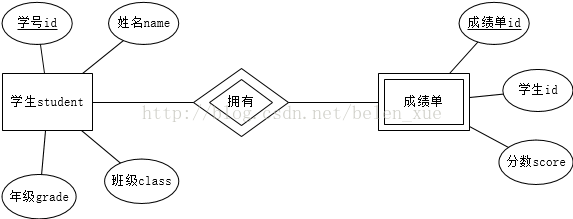
\includegraphics[width=\linewidth]{ER2.png}
\end{figure}

\begin{figure}[H]
    \centering
    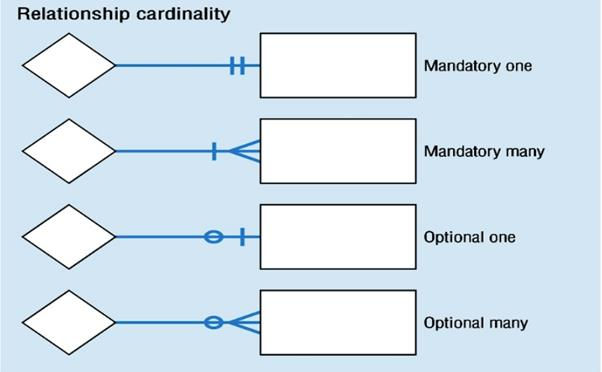
\includegraphics[width=\linewidth]{ER.jpg}
\end{figure}

Drawing steps

\begin{enumerate}
    \item Entity Identification: Identify entities
    \item Relationship Identification: Identify relationships
    \item Cardinality Identification: Identify cardinality (one-to-many, etc.)
    \item Identify Attributes: Identify columns
    \item Create ER Diagram: Draw the diagram
\end{enumerate}


\subsection{Data Warehouse}

Online Analytical Processing, using database systems to help gain insights into business, such as Redshift, primarily used for data analysis.

Data warehouses are optimized for read-only operations.

\begin{description}
    \item[Fact Table] Contains a large amount of data, can be summarized and recorded.
    
    \item[Dimension Table] Analyzes data from the perspective of attributes recorded in the fact table.
    
    \item[Star] Composed of one fact table and multiple dimension tables.
    
    \item[Snowflake] Each dimension table can be connected to multiple sub-dimension tables.
    
    \item[Galaxy] A version of the star schema with multiple fact tables sharing dimension tables in the model.
\end{description}

\subsubsection{Data Cube}

Represents large data sets, storing multi-dimensional data.

\begin{figure}[H]
    \centering
    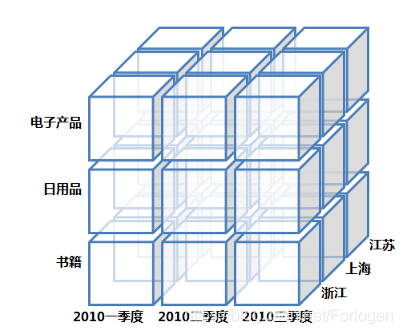
\includegraphics[width=\linewidth]{Cube.png}
\end{figure}

\begin{description}
    \item[Drill Down] Quarterly total sales $\to$ each month.
    
    \item[Roll Up] Months 4, 5, 6 $\to$ Second quarter.
    
    \item[Slice] Analyzing only electronic products.
    
    \item[Dice] First and second quarters.
    
    \item[Rotate] Exchange dimensions between products and regions.
\end{description}

\begin{figure}[H]
    \centering
    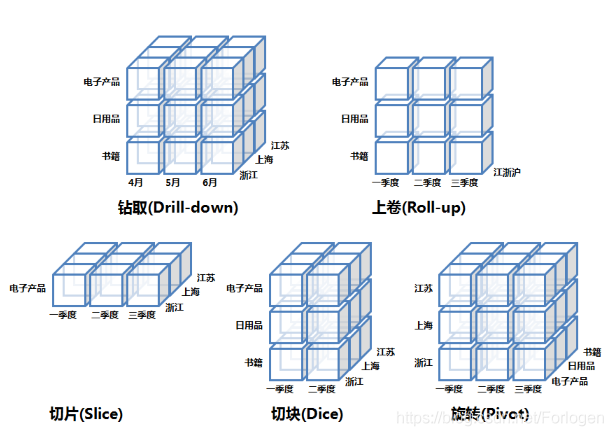
\includegraphics[width=\linewidth]{Action.png}
\end{figure}


\section{Algorithms \& Data Structures}


\subsection{The Concept of Algorithms, the Description of an Algorithm}

An algorithm is similar to a recipe, where each step is a specific action taken to achieve a goal. It includes a set of inputs, operates on the inputs, and produces outputs. It must be clearly defined, have a specific purpose, and be able to complete the task in a reasonable time using reasonable resources.


\subsection{Turing Machines}

\url{https://Aloen.to/Algorithm/TM/Turing-Machines/}

\begin{itemize}
    \item Abstract models for real computers with infinite memory (in the form of a tape) and a reading head.
    
    \item Has a finite number of internal states.
    
    \item Has distinguished starting and final states.
    
    \item Has transition functions.
\end{itemize}

\begin{itemize}
    \item Accepts the initial content of the tape if it terminates in an accepting state.
    
    \item If there is no matching rule, it terminates.
    
    \item If there are multiple matching rules for a state and input symbol set, it is non-deterministic.
    
    \item All non-deterministic machines have equivalent deterministic machines.
\end{itemize}


\subsubsection{Halting Problem}

Belongs to Computability Theory, determining if any program can finish running in a finite amount of time. The Traveling Salesman Problem is not in this category.


\subsection{Efficiency of Algorithms, Basics of Complexity Theory}

Algorithms consume time and memory; complexity measures these consumption indicators.


\subsubsection{Time Complexity}

The time complexity is mainly caused by loops, where \(O\) represents the trend of growth. The following complexities are listed in increasing order, indicating decreasing efficiency.

\begin{description}
    \item[Constant Time \(O(1)\)] ~

    \begin{minted}{js}
        let i = 1;
        i = i + 1;
    \end{minted}

    No loops involved.

    \item[Logarithmic Time \(O(\log N)\)] ~

    \begin{minted}{js}
        let i = 1;
        while (i < n)
          i = i * 2;
    \end{minted}

    After \(x\) iterations, \(i > n\), implying \(2^x > n\), i.e., \(x > \log_2 (n)\).

    \item[Linear Time \(O(N)\)] ~

    \begin{minted}{js}
        for (let i = 0; i < n; i++)
          console.log(i);
    \end{minted}

    Loops \(n\) times.

    \item[Linear Logarithmic Time \(O(N \log N)\)] ~

    \begin{minted}{js}
        for (let i = 1; i < n; i = i * 2)
          for (let j = 0; j < n; j++)
            console.log(j);
    \end{minted}

    Executes \(O(\log N)\) code \(N\) times or \(O(N)\) code \(\log N\) times.

    \item[Quadratic Time \(O(N^2)\)] ~

    \begin{minted}{js}
        for (let i = 0; i < m; i++)
          for (let j = 0; j < n; j++)
            console.log(j);
    \end{minted}

    Executes \(O(N)\) code \(N\) times or \(m \times n\).

\end{description}

Others include but are not limited to:

\begin{itemize}
    \item Polynomial Time \(O(N^k)\)

    \item Exponential Time \(O(2^N)\) (typically recursive algorithms)

    \item \(O(3^N)\)
\end{itemize}

\paragraph{Calculation} ~

\(T(n)\): Number of executions of the algorithm

\(T(n) = O(f(n))\)

\begin{description}
    \item[Nested Loops] ~

    Analyze from the innermost loop outward and multiply the complexities.

    \begin{minted}{js}
        // O(n)
        for (let i = 0; i < n; i++)
          // O(n)
          for (let j = 0; j < n; j++)
            console.log(j); // O(1)
    \end{minted}

    Time complexity is \(O(n \times n \times 1) = O(n^2)\).

    \item[Sequential Execution] ~

    Add the time complexities.

    \begin{minted}{js}
        // O(n)
        for (let i = 0; i < n; i++)
          console.log(i);

        // O(n^2)
        for (let i = 0; i < n; i++)
          for (let j = 0; j < n; j++)
            console.log(j);
    \end{minted}

     \(O(n + n^2)\) or \(O(n^2)\).

    \item[Conditional Branching] ~

    Consider the most complex scenario.

    \begin{minted}{js}
        if (n > 10)
          // O(n)
          for (let i = 0; i < n; i++)
            console.log(i);
        else
          // O(1)
          console.log(n);
    \end{minted}

    \(O(n)\)

\end{description}

\subsubsection{Space Complexity}

\begin{description}
    \item[Constant Space \(O(1)\)] ~

    \begin{minted}{js}
        let i = 1;
        i = i + 1;
    \end{minted}

    The space allocated for variables does not change with the size of the data.

    \item[Linear Space \(O(N)\)] ~

    \begin{minted}{js}
        let arr = [];
        for (let i = 0; i < n; i++)
          arr.push(i);
    \end{minted}

    Involves an array, and space increases with \(n\).
\end{description}

So, if \(n\) increases, the program's space usage:

\begin{itemize}
    \item Remains constant, \(O(1)\)

    \item Increases linearly, \(O(N)\)

    \item Increases quadratically, \(O(N^2)\)

\end{itemize}

And so on, also considering \(O(N + M)\), \(O(\log N)\), etc.


\subsection{Approaches to algorithm construction}

\begin{description}
    \item[Brute Force] Try all possible solutions until feasible; not necessarily efficient.
    
    \item[Divide and Conquer] Decompose the problem into multiple subproblems, solve each separately, and then combine.
    
    \item[Greedy] Make locally optimal choices at each step, but not necessarily globally optimal.
    
    \item[Dynamic Programming] Attempt to solve each subproblem only once to reduce computation, highly effective for problems with overlapping subproblems.
    
    \item[Backtracking] Explore all possible solutions incrementally, backtrack when incorrect.
    
    \item[Randomized] Use randomization to find approximate solutions to optimization problems.
\end{description}


\subsection{Linear data structures}

\begin{description}
    \item[Lists] A specific type of collection, ordered and may contain duplicates, implemented using arrays or linked lists.
    
    \item[Collections] Grouping of elements, may be ordered/unordered, contain duplicates/unique, includes various data structures like Set, Map, etc.
    
    \item[First-In-First-Out] Queue, follows the first-in-first-out principle.
    
    \item[Last-In-First-Out] Stack, follows the last-in-first-out principle.
    
    \item[Binary Heap] A complete binary tree filled from left to right.
\end{description}

\url{https://Aloen.to/Algorithm/Basics-of-Computer-Science/#Sorting-algorithms-and-their-complexity}


\subsection{Search in hash tables}

Store key-value pairs, O(1) time complexity, map data to its hash value.

Handling collisions:

\begin{description}
    \item[Separate Chaining] Store elements with the same hash value in a linked list; linear search is required when accessing this list, requiring additional space and time.
    
    \item[Open Addressing] If two elements have the same hash value, generate another hash value, prone to consecutive hash value occupation, not suitable for large datasets.
\end{description}


\subsection{Binary Search Tree}

In a binary search tree (BST):

\begin{itemize}
    \item All nodes in the left subtree are smaller than the root.
    
    \item All nodes in the right subtree are larger than the root.
    
    \item Every subtree is a binary search tree.
    
    \item No duplicate nodes are allowed.
\end{itemize}

\begin{figure}[H]
    \centering
    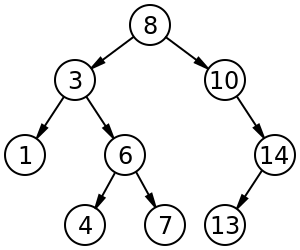
\includegraphics[width=0.5\linewidth]{BST.png}
\end{figure}

Searching in the tree involves comparing node values; the leftmost is the smallest, and the rightmost is the largest.


\subsubsection{Deleting a Node}

Deleting a node while maintaining the BST structure:

\begin{itemize}
    \item No child: Delete directly.
    
    \item Single child: Replace with the child.
    
    \item Both children: Replace with the successor node.
\end{itemize}

The successor node is the next node in an in-order traversal. To find A's successor, start from A's right subtree, and go left until there is no left child.


\subsection{234 / RB Tree}

BV1BB4y1X7u3 / BV1Ce4y1Q76H


\section{Graph Algorithms}


\subsection{The concept of a graph, its representations and visualization}

$G=(V,E)$ where V is a finite, non-empty set, V = edges, E = vertices.

Graph Representations:

\begin{itemize}
    \item Drawing
    \item Edge and Vertex List
    \item Adjacency Matrix
\end{itemize}

\begin{figure}
    \centering
    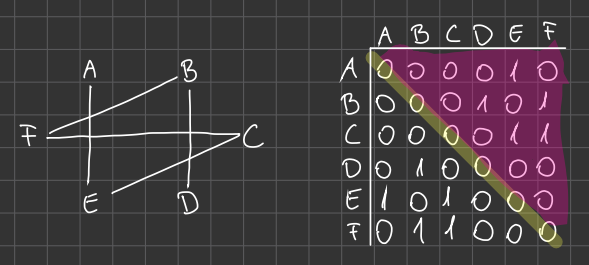
\includegraphics[width=\linewidth]{1.png}
\end{figure}


\subsection{Euler Path}

An Euler path, also known as the Eulerian path, is a solution to the "Seven Bridges of Königsberg" problem. A circuit, on the other hand, requires returning to the starting point. The path traverses each edge, and vertices can be visited multiple times.

For an undirected graph:

\begin{description}
    \item[Path] Nodes with odd degrees can have either 0 or 2 occurrences.
    
    \item[Circuit] No nodes with odd degrees are allowed.
\end{description}

For a directed graph:

\begin{description}
    \item[Path] Outdegree equals indegree or the starting node has one more outdegree than indegree, and the ending node has one more indegree than outdegree, with all other nodes having equal indegree and outdegree.
    
    \item[Circuit] Outdegree equals indegree for all nodes.
\end{description}

\subsubsection{Hierholzer}

Algorithm, $O(V + E)$:

\begin{enumerate}
    \item Start from a vertex with an Eulerian path.
    
    \item Perform a depth-first traversal of the entire graph, marking visited vertices.
    
    \item If a vertex has no unvisited neighbors, push it onto the stack and remove it.
\end{enumerate}

\subsection{Hamiltonian Path}

A Hamiltonian path emphasizes visiting each vertex once. It is an NP-complete problem, often solved using enumeration. Backtracking is a form of depth-first search that does not retain the complete tree structure during the solution process, in contrast to DFS, which records the entire search tree. The choice of the starting point is crucial for finding a path; for the same graph, a Hamiltonian path may exist starting from one vertex but not from another.

\subsection{Tree Graphs}

A tree is an undirected, acyclic connected graph where each pair of vertices is connected by a unique path.

\subsection{Fundamental graph algorithms}

\begin{description}
    \item[Pre] XLR
    \item[Mid] LXR
    \item[Post] LRX
\end{description}

\begin{figure}
    \centering
    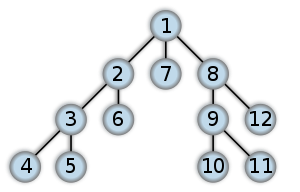
\includegraphics[width=\linewidth]{DFS.png}
    \caption{Depth-First Search}
\end{figure}

\begin{figure}
    \centering
    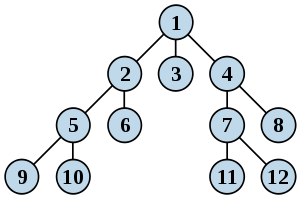
\includegraphics[width=\linewidth]{BFS.png}
    \caption{Breadth-First Search}
\end{figure}

\subsection{Optimal spanning trees}

The minimum spanning tree problem involves finding the smallest total weight tree in a weighted, undirected connected graph that spans all vertices.

\subsubsection{Prim}

Greedy algorithm, $O(V^2)$:

\begin{enumerate}
    \item Choose a vertex as the starting point.
    
    \item Select the minimum-weight edge adjacent to the current tree in each iteration.
\end{enumerate}

\url{https://en.wikipedia.org/wiki/Prim%27s_algorithm#Example}

\subsubsection{Kruskal}

Greedy algorithm, $O(E \log V)$:

\begin{enumerate}
    \item Sort all edges in ascending order.
    
    \item Iterate through edges, adding them to the tree if their connecting nodes are not in the same connected component.
\end{enumerate}

\url{https://en.wikipedia.org/wiki/Kruskal%27s_algorithm#Example}

\subsection{Shortest paths}

Shortest path algorithms find the most efficient route between two vertices in a graph with weighted edges.


\subsubsection{Dijkstra}

\begin{minted}{js}
A --5-- B
|       |
4       6
|       |
C --5-- D
\end{minted}

First, set A as the origin and initialize the distance from each vertex to the origin as \infty

\begin{minted}{js}
/** Distance from each vertex to the origin */
let dist: Record<string, number> = {
  A: 0,
  B: Infinity,
  C: Infinity,
  D: Infinity,
};

/** Get the weight between two vertices */
declare function weight(node1: string, node2: string): number;
\end{minted}

Next, iteratively update the shortest distance from each point to the origin. In each iteration, find the closest point to the origin among those not yet updated, then update its shortest distance to the origin. Based on the new distance, update the distances from other points to the origin.

Expanding from A:

\begin{minted}{js}
dist.B =
  Math.min(dist.B, dist.A + weight("A", "B")) =
  Math.min(Infinity, 0 + 5) =
    5;

dist.C =
  Math.min(dist.C, dist.A + weight("A", "C")) =
  Math.min(Infinity, 0 + 4) =
    4;
\end{minted}

Expanding from B:

\begin{minted}{js}
dist.D =
  Math.min(dist.D, dist.B + weight("B", "D")) =
  Math.min(Infinity, 5 + 6) =
    11;
\end{minted}

Expanding from C:

\begin{minted}{js}
dist.D = 
  Math.min(dist.D, dist.C + weight("C", "D")) = 
  Math.min(11, 4 + 5) = 
    9;
\end{minted}

Result:

\begin{minted}{js}
dist = {
  A: 0,
  B: 5,
  C: 4,
  D: 9,
};
\end{minted}

So, the shortest distance from A to D is 9


\subsection{Bellman-Ford}

Finding the shortest paths in a graph with negative weights, iterate over the entire graph V - 1 times, reducing distances whenever possible.

BV1j34y1s7d8


\section{Programming}


\subsection{Arithmetical and logical operations}

\begin{description}
    \item[Arithmetic] \verb|+ - * / % ++ --|

    \item[Relational] \verb|== != > < >= <=|

    \item[Logical] \verb|&&| || !

    \item[Bitwise] \& | ~ \verb|^ << >>|

    \item[Assignment] \verb|= += -= *= /=|
\end{description}


\subsection{Control structures (conditional and unconditional flow control, loops)}

\begin{description}
    \item[Conditional statements] if else switch

    \item[Loops] for in of do while break continue
\end{description}


\subsection{Functions and procedures (subprograms, subroutines)}

Function: Subprograms, reuse code blocks, perform specific tasks

Procedure: Subroutine, does not return a value, achieves tasks through side effects


\subsection{data passing}

\begin{description}
    \item[Pass by value] Pass a copy
    \item[Pass by reference] Pass a pointer
    \item[ref] Pass by reference for value types 
    \item[int[]] Pass by value for reference types 
\end{description}


\subsection{local and global variables}

\begin{description}
    \item[Local] Declared within a scope, gets destroyed

    \item[Global] Accessible from any part
\end{description}


\subsection{the role of stacks in function calls}

Call Stack is a structure managing function call relationships, ensuring order and tracking


\subsubsection{Stack Frame}

Function parameters and local variables are stored in the Stack Frame, pushed onto the Call Stack, and popped out after execution. It contains the function's execution environment, including: Function Parameters, Local Variables, Return Address


\subsubsection{Function Call}

When a function is called,

\begin{enumerate}
    \item Push the return address (instruction after function execution) onto the stack.
    \item Push arguments onto the stack.
    \item Jump to the starting position of the function, entering the function.
    \item Create a new Stack Frame with locally allocated variables.
    \item Execute the function.
\end{enumerate}


\subsubsection{Function Return}

When a function has completed its execution and is ready to return,

\begin{enumerate}
    \item If the function has a return value, store it in a specific location for the caller to access.
    \item Pop the function's frame from the call stack, destroying local variables and arguments.
    \item Jump to the return address and continue execution.
\end{enumerate}


\subsubsection{Recursion}

When a function directly or indirectly calls itself, each call creates a new Stack Frame. The size of the call stack is limited. If the recursion depth is too high or there are too many function calls, the call stack may overflow.


\subsection{Basics of Object-Oriented Programming: Classes, Objects, Inheritance, Polymorphism, Encapsulation}

\begin{description}
    \item[Objects] are instances of classes.
    
    \item[Polymorphism] allows an object to take on multiple forms, often achieved through virtual, abstract, or interface methods for reusability and flexibility.
    
    \item[Encapsulation] involves encapsulating data and related behaviors within a class, hiding implementation details from external access using access modifiers.
\end{description}


\section{Compilers}


\subsection{Chomsky Classification}

\begin{table}[H]
\centering
\begin{tabular}{|c|c|c|c|}
\hline
Grammar & Language & Type & Production Rules \\
\hline
0 & Recursively Enumerable & Turing Machine & $\alpha \rightarrow \beta$ \\
\hline
1 & Context-Sensitive & Linear Bounded Non-deterministic Turing & $\alpha A \beta \rightarrow \alpha \gamma \beta$ \\
\hline
2 & Context-Free & Non-deterministic Pushdown Automaton & $A \rightarrow \gamma$ \\
\hline
3 & Regular & Finite State Automaton & $A \rightarrow aB$ \\
& & & $A \rightarrow a$ \\
\hline
\end{tabular}
\end{table}


\subsection{Regular Languages}

\begin{itemize}
    \item The empty set Ø is a regular language.
    \item A language containing only the empty string $\epsilon$ is a regular language.
\end{itemize}


\subsection{Relation to Lexical Analyzer Programs}

A Tokenizer breaks a sequence of symbols into a sequence of tokens, which are then passed to the Parser to generate an Abstract Syntax Tree (AST).

Regular languages can describe patterns and rules defining programming language symbols, and regular expressions are one way to express these patterns.

[Link to additional resource](https://juejin.cn/post/6844904035271573511)


\subsection{Finite Automata}

Finite-State Machines are used to recognize regular languages.

\begin{description}
    \item[Deterministic] Each state and input has a determinate next state.
    
    \item[Nondeterministic] Can transition to different next states, may have $\epsilon$ transitions that do not consume input.
\end{description}


\subsection{The Structure of Compilers}

Translation of high-level code to low-level language involves:

\begin{description}
    \item[Lexical] Lexical analysis.
    \item[Syntax] Syntax analysis, AST generation.
    \item[Semantic] Checking for syntax correctness, type checking, etc.
    \item[Intermediate] Platform-independent intermediate code.
    \item[Optimization] Performance improvements, etc.
    \item[Generation] Generation of target machine code.
\end{description}


\subsection{The Process of Compilation or Interpretation}

\begin{description}
    \item[Compilation] Code is translated into machine code before execution, resulting in faster execution.
    
    \item[Interpretation] Source code is executed directly (e.g., JavaScript), potentially slower.
\end{description}

Languages like Java use Intermediate Language (IL) for pre-compilation.


\subsection{Look-Ahead}

During the parsing phase, predicting input based on the parser's current state helps determine which rule to apply in case of ambiguity. Understanding more complex grammars, where k represents the number of tokens that can be looked ahead:

\begin{description}
    \item[LL(k)] Top-down, Left-to-right, Leftmost derivation.
    
    \item[LR(k)] Bottom-up, Left-to-right, Rightmost derivation.
\end{description}


\section{System Engineering}


\subsection{Basics of UML}

Unified Modeling Language, which uses graphical symbols to describe system structure, behavior, and interactions.

\begin{description}
    \item[Class] Represents attributes, methods, relationships, constraints, and static structures.
    
    \item[Object] Represents a snapshot or instance of a class.

    \item[Use Case] Describes interactions between actors and system functionalities.

    \item[Sequence] Illustrates interactions between objects over time.

    \item[Component] Represents modules, libraries, and dependencies.
\end{description}


\subsection{Meta-models}

The underlying framework or language used to define and describe the constructs and rules of UML. It defines the syntax and semantics of UML for interpreting models.


\subsection{The 4-layer meta-model of UML}

\begin{description}
    \item[M0] Run-Time instances, representing concrete objects and data existing during actual execution.

    \item[M1] User model, representing users' understanding of the system, interactions, expectations, goals, and tasks.

    \item[M2] UML abstraction, used to define meta models.

    \item[M3] Meta-Object Facility, the highest level of abstraction.
\end{description}


\subsection{Basics of workflow modeling}

\begin{description}
    \item[Identify Boundaries] Specify the content, scope, inputs, outputs, etc., to be modeled.

    \item[Define Objectives] Determine modeling goals, expected results, constraints, etc.

    \item[Identify Components] Determine the components involved.

    \item[Establish Relationships] Identify relationships and dependencies.

    \item[Model Structure] Use graphical symbols to represent the structure.

    \item[Specify Logic] Determine conditions, loops, exception handling, etc.

    \item[Iterate and Refine] Continue refining the model.
\end{description}


\subsection{The Software Process Engineering Model (SPEM) UML profile describes the classic and RUP methodologies steps}

\subsubsection{Classic Waterfall}

\begin{description}
    \item[Requirements Analysis] 

    \item[System Design] 

    \item[Implementation] 

    \item[Testing and Integration] 

    \item[Deployment] 

    \item[Operation and Maintenance] 
\end{description}


\subsubsection{Rational Unified Process}

\begin{description}
    \item[Inception] Determine scope, goals, risks, proposals, feasibility.

    \item[Elaboration] Establish priorities, design system architecture, plan.

    \item[Construction] Implement the system, test, review.

    \item[Transition] Acceptance testing, deployment.
\end{description}


\subsection{Programming and software engineering technologies and methodologies}

\begin{description}
    \item[Programming Languages] Java
    
    \item[Integrated Development Environments] VS IDEA

    \item[Version Control Systems] GIT

    \item[Agile Methodologies] Kanban

    \item[DevOps] Continuous Integration / Delivery

    \item[Software Development Lifecycle] Waterfall
\end{description}


\subsection{Procedural techniques}

Programming paradigms, where OOP is one.

\begin{description}
    \item[Modular Programming] ~

    \begin{itemize}
        \item Modularization
        \item Encapsulation
    \end{itemize}

    \item[Control Structures] ~

    \begin{itemize}
        \item Sequence
        \item Selection
        \item Iteration
    \end{itemize}

    \item[Abstraction] 

    \item[Variable Scope and Lifetime] 

    \item[Error Handling] 
\end{description}


\end{document}
